\documentclass{beamer}
% http://deic.uab.es/~iblanes/beamer_gallery/index_by_theme.html
\mode<presentation>
{
    \usetheme{Montpellier}
    \usecolortheme{dolphin}
    \usefonttheme{default}
    \setbeamertemplate{navigation symbols}{}
    \setbeamertemplate{caption}[numbered]
} 

\usepackage[english]{babel}
\usepackage[utf8]{inputenc}
\usepackage[T1]{fontenc}
\usepackage{graphicx, tikz}
\usepackage[framemethod=TikZ]{mdframed}

%amsmath

\newcommand\annotatedFigureBoxCustom[8]{
    \draw[#5,ultra thick,rounded corners] (#1) rectangle (#2);
    \node at (#4) [fill=#6,thick,shape=circle,draw=#7,
                   inner sep=2pt,font=\sffamily,text=#8]
                   {\textbf{#3}};
}


% {from}{to}{text}{color}
\newcommand\anbox[4]{\annotatedFigureBoxCustom{#1}{#2}{#3}{#1}{#4}{white}{black}{black}}


\newcommand\antext[5]{
    \draw[#4, fill=#5, ultra thick, rounded corners] (#1) rectangle (#2)
    node[pos=0.5, font=\sffamily, text=black] {\textbf{#3}};
}


\newenvironment{anfig}[1]
{
    \begin{mdframed}[linecolor=blue!65!white, linewidth=2pt, roundcorner=0.75pt,
                     innerrightmargin=0.05pt, innerleftmargin=0.05pt,
                     innertopmargin=0.05pt, innerbottommargin=0.05pt, frametitle={}]
    \begin{tikzpicture}
    \node[anchor=south west,inner sep=0] (image) at (0,0)
    {\includegraphics[width=\textwidth]{#1}};
    \begin{scope}[x={(image.south east)},y={(image.north west)}]
}
{
    \end{scope}
    \end{tikzpicture}
    \end{mdframed}
}

\def\fcol{\color{blue!55!black}}

\newcommand{\fig}[1]{
    \begin{mdframed}[linecolor=blue!65!white, linewidth=1.75pt, roundcorner=0.75pt,
                     innerrightmargin=0pt, innerleftmargin=0pt,
                     innertopmargin=0pt, innerbottommargin=0pt,
                     backgroundcolor=white, frametitle={}, align=center]
        \includegraphics[width=1.0\textwidth]{#1}
    \end{mdframed}
}

\newcommand{\figm}[2]{
    \begin{center}
    \begin{minipage}[c]{#2\textwidth}
    \begin{mdframed}[linecolor=blue!65!white, linewidth=1.75pt, roundcorner=0.75pt,
                     innerrightmargin=0pt, innerleftmargin=0pt,
                     innertopmargin=0pt, innerbottommargin=0pt,
                     backgroundcolor=white, frametitle={}, align=center]
        \includegraphics[width=1.0\textwidth]{#1}
    \end{mdframed}
    \end{minipage}
    \end{center}
}

\newenvironment{minic}[1]
{
    \begin{center}
    \begin{minipage}[c]{#1\textwidth}
}
{
    \end{minipage}
    \end{center}
}


\newenvironment{figp}[4]
{
    \begin{minipage}[c]{#3\textwidth}
    \centering
    #1
    
    #2
    \end{minipage}
    \begin{minipage}[c]{#4\textwidth}
}
{
    \end{minipage}
}


\newcommand{\figc}[2]
{
    \begin{center}
    \begin{mdframed}[linecolor=blue!65!white, linewidth=1.75pt, roundcorner=0.75pt,
                     innerrightmargin=0pt, innerleftmargin=0pt,
                     innertopmargin=0pt, innerbottommargin=0pt,
                     backgroundcolor=white, frametitle={}, align=center]
    
    \includegraphics[width=1.0\textwidth]{#1}
    \end{mdframed}
    #2
    \end{center}
}

\newcommand\sepframe[1] {
    \begin{frame}
        \begin{center}
            \Huge \fcol
            #1
        \end{center}
    \end{frame}
}

\newcommand\bench[2]{
    \begin{minipage}[t]{0.45\textwidth}
        \centering
        \includegraphics[width=\textwidth]{#1}
        \vspace{7.5pt}
        
        LOS deformáció.
    \end{minipage}
    \hspace{5pt}
    \begin{minipage}[t]{0.45\textwidth}
        \centering
        \includegraphics[width=\textwidth]{#2}
        \vspace{7.5pt}
        
        Kálmán-szűréssel integrált GNSS és InSAR mérések.
    \end{minipage}
}

\def\boxcolor{black}
\def\fillcolor{white}
\def\refcolor{orange}


\def\hun{
    \begin{anfig}{hungary_networks_raw.png}
        \anbox{0.27, 0.3}{0.33, 0.4}{A}{\boxcolor}
        \anbox{0.5, 0.4}{0.5525, 0.525}{B}{\boxcolor}
        \anbox{0.465, 0.05}{0.535, 0.15}{C}{\boxcolor}
    \end{anfig}
}

\def\erdely{
    \begin{anfig}{transylvania_networks_raw.png}
        \anbox{0.4075, 0.55}{0.4875, 0.67}{A}{\boxcolor}
        \anbox{0.55, 0.37}{0.63, 0.49}{B}{\boxcolor}
        \anbox{0.75, 0.08}{0.9, 0.4}{C}{\boxcolor}
    \end{anfig}
}

\def\dszekcso{
    \begin{anfig}{dszekcso_network_raw.png}
        \antext{0.05, 0.57}{0.25, 0.64}{IB1}{\refcolor}{\fillcolor}
        \antext{0.3, 0.67}{0.5, 0.74}{IB2}{\boxcolor}{\fillcolor}
        \antext{0.225, 0.47}{0.425, 0.54}{IB3}{\boxcolor}{\fillcolor}
        \antext{0.32, 0.25}{0.52, 0.32}{IB4}{\boxcolor}{\fillcolor}
    \end{anfig}
}

\def\kulcs{
    \begin{anfig}{kulcs_network_raw.png}
        \antext{0.125, 0.875}{0.225, 0.975}{A1}{\boxcolor}{\fillcolor}
        \antext{0.51, 0.45}{0.61, 0.55}{A2}{\boxcolor}{\fillcolor}
        \antext{0.825, 0.17}{0.925, 0.27}{A3}{\boxcolor}{\fillcolor}
        \antext{0.79, 0.04}{0.89, 0.14}{A4}{\boxcolor}{\fillcolor}
        \antext{0.46, 0.17}{0.56, 0.27}{AR}{\refcolor}{\fillcolor}
        \antext{0.475, 0.7}{0.625, 0.8}{Duna}{\boxcolor}{\fillcolor}
    \end{anfig}
}

\def\fonyod{
    \begin{anfig}{fonyod_network_raw.png}
        \antext{0.25, 0.78}{0.45, 0.86}{Balaton}{\boxcolor}{\fillcolor}
        \antext{0.725, 0.77}{0.825, 0.87}{KV}{\boxcolor}{\fillcolor}
        \antext{0.725, 0.16}{0.825, 0.26}{PH}{\refcolor}{\fillcolor}
        \antext{0.29, 0.0575}{0.39, 0.1575}{RE}{\boxcolor}{\fillcolor}
    \end{anfig}
}


\def\csomad{
    \begin{anfig}{ciomadul_network_raw.png}
        \antext{0.3, 0.29}{0.42, 0.375}{C1}{\boxcolor}{\fillcolor}
        \antext{0.21, 0.1}{0.33, 0.18}{C2}{\refcolor}{\fillcolor}
        \antext{0.665, 0.2}{0.775, 0.28}{C3}{\boxcolor}{\fillcolor}
        \antext{0.49, 0.565}{0.6, 0.645}{C4}{\boxcolor}{\fillcolor}
        \antext{0.64, 0.82}{0.76, 0.9}{C5}{\refcolor}{\fillcolor}
    \end{anfig}
}



\graphicspath{{../../images/}}

\title[InSAR]{Theoretical background of artificial radar interferometry benchmarks and preliminary results}
\author{István Bozsó, Eszter Szűcs, László Bányai, Viktor Wesztergom}
\institute{MTA CSFK Geodetic and Geophysical Institute}
\date{2018.10.28.}


\begin{document}

\begin{frame}
    \titlepage
    \begin{center}
        \begin{minipage}[c]{0.25\textwidth}
            
\includegraphics[width=0.75\textwidth]{ggi_logo.png}
        \end{minipage}
        \hspace{30pt}
        \begin{minipage}[c]{0.25\textwidth}
            
\includegraphics[width=0.75\textwidth]{esa_logo.eps}
        \end{minipage}
    \end{center}
\end{frame}

\begin{frame}{Outline}
    \tableofcontents
\end{frame}


\section{Introduction}

\begin{frame}{Introduction}
    \begin{itemize}
    \large
        \item no natural scatterers $\rightarrow$ no deformation time series from that area $\rightarrow$ we need artificial reflectors
        \item parameters to be determined: size, geometry and placement of reflectors
            \begin{itemize}
            \large
                \item size and geometry from electromagnetic properties
                \item placement based on information gathered from field trips
            \end{itemize}
    \end{itemize}
    
\end{frame}


\section{The theory behind artificial reflectors}

\begin{frame}{Design of artificial reflectors}
    \begin{itemize}
        \item analogue, analytical and numerical calculations,
        \item Sentinel-1 observing wavelength and orbit parameters,
        \item mechanical compactness and robustness.
    \end{itemize}
    \begin{center}
        \resizebox{0.1\textwidth}{30pt}{$\Downarrow$}
        \vspace{10pt}
        
        optimal reflector geometry
    \end{center}
\end{frame}


\subsection{Phase unwrapping}

\begin{frame}{Phase unwrapping}
    \begin{center}
        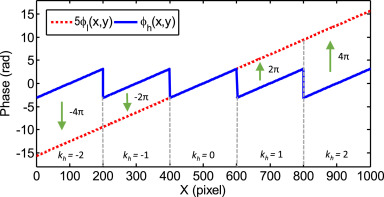
\includegraphics[width=0.8\textwidth]{phase_unwrapping.jpg}
    \end{center}
\end{frame}


\subsection{Geometry of satellite orbits}

\begin{frame}{Geometry of satellite orbits}
    \begin{minipage}[c]{0.45\textwidth}
        \centering
        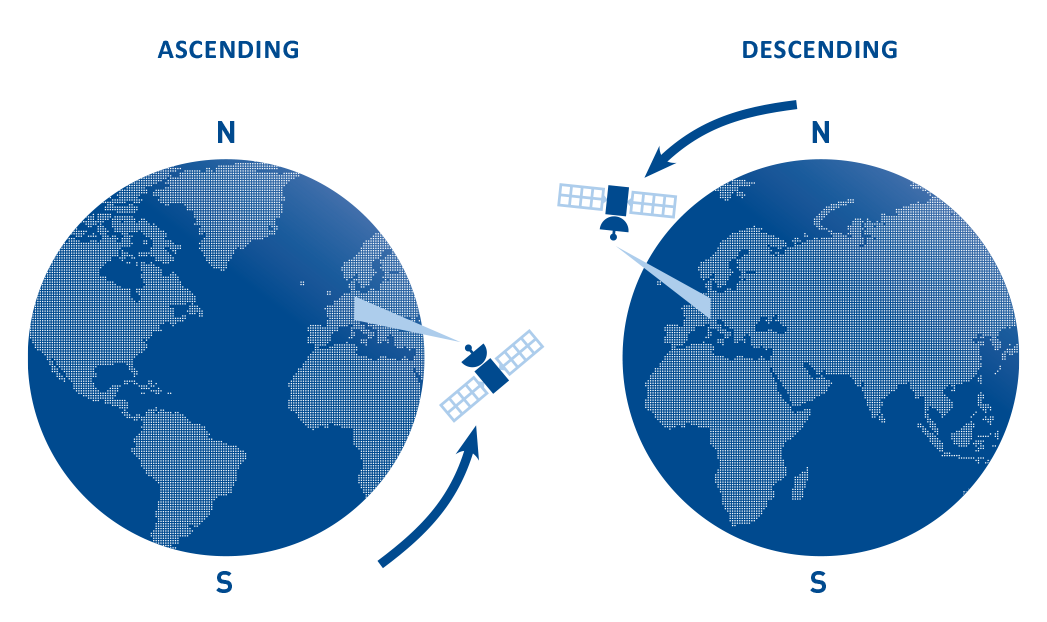
\includegraphics[width=\textwidth]{ascending_descending_orbits.png}
        
        Ascending and descending satellite orbits.
    \end{minipage}
    \hspace{10pt}
    \begin{minipage}[c]{0.45\textwidth}
        \centering
        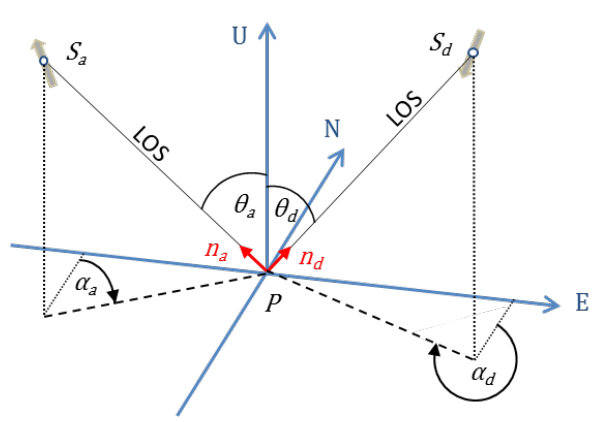
\includegraphics[width=\textwidth]{daisy_schematic.png}
        
        Geometry of ascending and descending satellite orbits and reflector postisions
    \end{minipage}
\end{frame}


\subsection{Integration of GNSS and interferometric measurements}


\begin{frame}{Kalman-filtering}
    \begin{itemize}
        \item \textbf{InSAR}
        \begin{itemize}
            \item only 2 independent measurements $\rightarrow$ only 2D (east-west and vertical)
            \item every 6 days
        \end{itemize}
        \item \textbf{GNSS}
        \begin{itemize}
            \item 3D movements
            \item not cost effective to make measurements very often
        \end{itemize}
    \end{itemize}
    \vspace{10pt}
    \begin{center}
        combine GNSS and InSAR with Kalman-filtering
        
        \resizebox{0.1\textwidth}{30pt}{$\Downarrow$}
        \vspace{10pt}
        
        3D movements every 6 days
    \end{center}
\end{frame}


\section{First results of reflector benchmarks}

\sepframe{Reflector networks in Hungary and first results}

\begin{frame}{Installed reflectors in Hungary}
    \begin{minipage}[c]{0.7\textwidth}
        \begin{anfig}{hungary_networks_raw.png}
            \anbox{0.27, 0.3}{0.33, 0.4}{A}{\boxcolor}
            \anbox{0.5, 0.4}{0.5525, 0.525}{B}{\boxcolor}
            \anbox{0.465, 0.05}{0.535, 0.15}{C}{\boxcolor}
        \end{anfig}
    \end{minipage}
    \hspace{5pt}
    \begin{minipage}[c]{0.25\textwidth}
         \textbf{A}: Fonyód\\
         \textbf{B}: Kulcs\\
         \textbf{C}: Dunaszekcső
    \end{minipage}
\end{frame}


\begin{frame}{Installed reflectors in Hungary}
    \begin{minipage}[c]{0.365\textwidth}
        \centering
        \begin{anfig}{dszekcso_network_raw.png}
            \antext{0.05, 0.55}{0.25, 0.65}{IB1}{\refcolor}{\fillcolor}
            \antext{0.3, 0.65}{0.5, 0.75}{IB2}{\boxcolor}{\fillcolor}
            \antext{0.225, 0.45}{0.425, 0.55}{IB3}{\boxcolor}{\fillcolor}
            \antext{0.32, 0.24}{0.52, 0.34}{IB4}{\boxcolor}{\fillcolor}
        \end{anfig}

        Dunaszekcső network
    \end{minipage}
    \hspace{10pt}
    \begin{minipage}[c]{0.58\textwidth}
        \centering
        \begin{anfig}{kulcs_network_raw.png}
            \antext{0.125, 0.875}{0.225, 0.975}{A1}{\boxcolor}{\fillcolor}
            \antext{0.51, 0.45}{0.61, 0.55}{A2}{\boxcolor}{\fillcolor}
            \antext{0.825, 0.17}{0.925, 0.27}{A3}{\boxcolor}{\fillcolor}
            \antext{0.79, 0.04}{0.89, 0.14}{A4}{\boxcolor}{\fillcolor}
            \antext{0.46, 0.17}{0.56, 0.27}{AR}{\refcolor}{\fillcolor}
            \antext{0.425, 0.7}{0.675, 0.8}{Danube}{\boxcolor}{\fillcolor}
        \end{anfig}
        Kulcs network
    \end{minipage}
\end{frame}


% ***************
% * Dunaszekcső *
% ***************


\begin{frame}{Dunaszekcső network IB2-IB1}
    \bench{IB2-IB1_los.png}{IB2-IB1_kalman.png}
\end{frame}

\begin{frame}{Dunaszekcső network IB3-IB1}
    \bench{IB3-IB1_los.png}{IB3-IB1_kalman.png}
\end{frame}

\begin{frame}{Dunaszekcső network IB4-IB1}
    \bench{IB4-IB1_los.png}{IB4-IB1_kalman.png}
\end{frame}


\begin{frame}{Installed reflectors in Hungary}
    \begin{minipage}[c]{0.365\textwidth}
        \centering
        \begin{anfig}{dszekcso_network_raw.png}
            \antext{0.05, 0.55}{0.25, 0.65}{IB1}{\refcolor}{\fillcolor}
            \antext{0.3, 0.65}{0.5, 0.75}{IB2}{\boxcolor}{\fillcolor}
            \antext{0.225, 0.45}{0.425, 0.55}{IB3}{\boxcolor}{\fillcolor}
            \antext{0.32, 0.24}{0.52, 0.34}{IB4}{\boxcolor}{\fillcolor}
        \end{anfig}

        Dunaszekcső network
    \end{minipage}
    \hspace{10pt}
    \begin{minipage}[c]{0.58\textwidth}
        \centering
        \begin{anfig}{kulcs_network_raw.png}
            \antext{0.125, 0.875}{0.225, 0.975}{A1}{\boxcolor}{\fillcolor}
            \antext{0.51, 0.45}{0.61, 0.55}{A2}{\boxcolor}{\fillcolor}
            \antext{0.825, 0.17}{0.925, 0.27}{A3}{\boxcolor}{\fillcolor}
            \antext{0.79, 0.04}{0.89, 0.14}{A4}{\boxcolor}{\fillcolor}
            \antext{0.46, 0.17}{0.56, 0.27}{AR}{\refcolor}{\fillcolor}
            \antext{0.425, 0.7}{0.675, 0.8}{Danube}{\boxcolor}{\fillcolor}
        \end{anfig}
        Kulcs network
    \end{minipage}
\end{frame}


% *********
% * Kulcs *
% *********


\begin{frame}{Kulcs network A1-AR}
    \bench{A1-AR_los.png}{A1-AR_kalman.png}
\end{frame}

\begin{frame}{Kulcs network A2-AR}
    \bench{A2-AR_los.png}{A2-AR_kalman.png}
\end{frame}

\begin{frame}{Kulcs network A3-AR}
    \bench{A3-AR_los.png}{A3-AR_kalman.png}
\end{frame}

\begin{frame}{Kulcs network A4-AR}
    \bench{A4-AR_los.png}{A4-AR_kalman.png}
\end{frame}


\begin{frame}{Installed reflectors in Hungary}
    \begin{minipage}[c]{0.6\textwidth}
        \centering
        \begin{anfig}{fonyod_network_raw.png}
            \antext{0.15, 0.77}{0.55, 0.87}{Lake Balaton}{\boxcolor}{\fillcolor}
            \antext{0.725, 0.77}{0.825, 0.87}{KV}{\boxcolor}{\fillcolor}
            \antext{0.725, 0.16}{0.825, 0.26}{PH}{\refcolor}{\fillcolor}
            \antext{0.29, 0.0575}{0.39, 0.1575}{RE}{\boxcolor}{\fillcolor}
        \end{anfig}

        Fonyód network
    \end{minipage}
    \hspace{5pt}
    \begin{minipage}[c]{0.3\textwidth}
            \textbf{PH}: Mayor's office\\
            \textbf{RE}: Ripka Memorial\\
            \textbf{KV}: Vault Villa
    \end{minipage}
\end{frame}


% **********
% * Fonyód *
% **********

\begin{frame}{Fonyód network KV-PH}
    \bench{KV-PH_los.png}{KV-PH_kalman.png}
\end{frame}

\begin{frame}{Fonyód network RE-PH}
    \bench{RE-PH_los.png}{RE-PH_kalman.png}
\end{frame}



\section{Installed and planned networks in Transylvania}

\sepframe{Reflector networks in Transylvania}

\begin{frame}{Installed reflectors in Transylvania}
    \begin{minipage}[c]{0.95\textwidth}
        \centering
        \begin{anfig}{transylvania_networks_raw.png}
            \anbox{0.4075, 0.55}{0.4875, 0.67}{A}{\boxcolor}
            \anbox{0.55, 0.37}{0.63, 0.49}{B}{\boxcolor}
            \anbox{0.75, 0.08}{0.9, 0.4}{C}{\boxcolor}
        \end{anfig}
            \textbf{A}: Praid network, 
            \textbf{B}: Ciomadul network, 
            \textbf{C}: Vrancea zone
    \end{minipage}
    %\hspace{5pt}
    %\begin{minipage}[c]{0.25\textwidth}
            %\textbf{A}: Praid network\\
            %\textbf{B}: Ciomadul network\\
            %\textbf{C}: Vrancea zone
        %\end{minipage}
\end{frame}


\begin{frame}{Praid network}
    \begin{minipage}[c]{0.7\textwidth}
        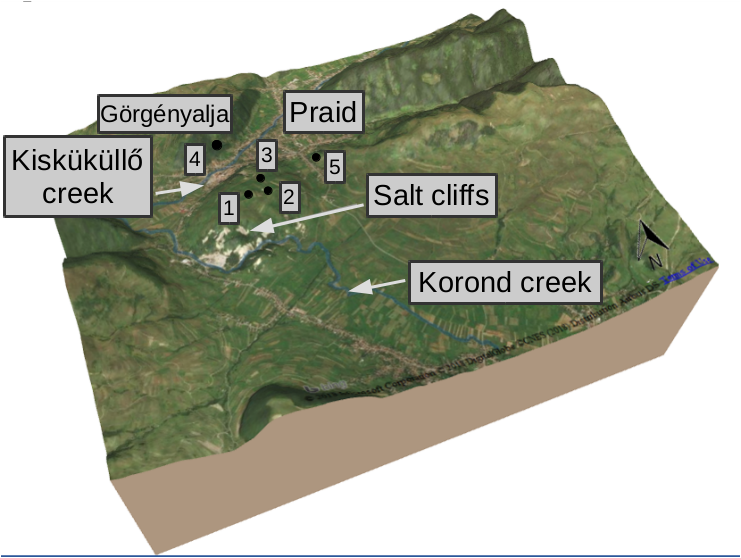
\includegraphics[width=\textwidth]{parajd_3D_mod.png}
    \end{minipage}
    \hspace{5pt}
    \begin{minipage}[c]{0.225\textwidth}
        \begin{itemize}
            \item largest salt diapir in Central-Europe $\rightarrow$ salt tectonics
            \item vertical movements?
        \end{itemize}
    \end{minipage}
\end{frame}


\begin{frame}{Praid network}
    \begin{minipage}[c]{0.75\textwidth}
        \ffig{praid_refl.png}
    \end{minipage}
    \hspace{10pt}
    \begin{minipage}[c]{0.195\textwidth}
        View from Reflector 5 (Catholic graveyard).
    \end{minipage}
\end{frame}


\begin{frame}{Ciomadul network}
    \begin{minipage}[c]{0.65\textwidth}
        \centering
        \ffig{ciomadul_network_raw.png}
    \end{minipage}
    \hspace{5pt}
    \begin{minipage}[c]{0.3\textwidth}
        \begin{itemize}
            \item magnetotelluric measurements indicate potentially active magma chamber
            \item possible movements in the vicinity of the Ciomadul volcano
        \end{itemize}
    \end{minipage}
\end{frame}


\begin{frame}{Conclusions}
    \begin{itemize}
        \item It is possible to monitor slow geodynamic processes with artificial corner reflectors.
        \item Reflector networks in Transylvania:
        \begin{itemize}
            \item Praid: ready
            \item Ciomadul: concrete foundations ready; reflectors need to be 
            \item Vrancea zone: suitable areas for reflector placement are needed.
        \end{itemize}
    \end{itemize}
\end{frame}


\begin{frame}
    \begin{center}
        \Huge \color{blue!55!black}
        Thank you for your attention!
    \end{center}
    \vspace{35pt}
    {\large
    Acknowledgement: Contains modified Copernicus Sentinel-1 data [2018]
    }
\end{frame}

\end{document}
